\documentclass[conference, a4paper]{IEEEtran}

\usepackage{cite}
\usepackage{amsmath,amssymb,amsfonts}
\usepackage{algorithmic}
\usepackage{graphicx}
\usepackage{textcomp}
\usepackage{xcolor}
\usepackage{hyperref} % Para enlaces y referencias cruzadas
\usepackage{fancyhdr} % Para controlar los encabezados y pies de página
\usepackage{float} % Para usar el modificador H en figuras

% Agregar números de página
\pagestyle{plain}

\begin{document}

\title{Programa MPI simple y caracterización del rendimiento}
\author{
    \IEEEauthorblockN{Jorge Otero y Pablo Seijo}
    \IEEEauthorblockA{Fundamentos de Sistemas Paralelos\\
    Universidad de Santiago de Compostela\\
    Email: pablo.garcia.seijo@rai.usc.es, jorge.otero.pailos@rai.usc.es }
}
\date{\today}

\maketitle

\begin{abstract}
En esta práctica se aborda la implementación y el análisis de un programa paralelo con MPI para calcular el valor de \(\pi\) mediante el método de Monte Carlo. Se evaluó el rendimiento en términos de tiempo de ejecución, eficiencia y calidad de los resultados al variar el número de procesos y el número de iteraciones. Los experimentos demuestran que el método es escalable y que la eficiencia mejora conforme aumenta el tamaño del problema.
\end{abstract}

% Agregar las palabras clave
\begin{IEEEkeywords}
MPI, Monte Carlo, paralelismo, eficiencia, speed-up, escalabilidad.
\end{IEEEkeywords}

\section{Introducción}
El cálculo de \(\pi\) ha sido objeto de estudio en numerosos contextos computacionales, especialmente por su importancia en pruebas de rendimiento de algoritmos paralelos. En esta práctica, se implementa un programa en C utilizando MPI para paralelizar el cálculo de \(\pi\) mediante el método de Monte Carlo. Se analizan el tiempo de ejecución, la eficiencia y la calidad de los resultados, que se mide como la inversa del producto entre el tiempo y el error.

La fórmula específica a analizar es la siguiente:

\begin{equation}
\pi = \frac{22}{7} - \int_{0}^{1} \frac{x^4 (1 - x)^4}{(1 + x)^2} \, dx
\end{equation}

Esta expresión presenta un enfoque alternativo para calcular \(\pi\) mediante métodos numéricos, lo que permite evaluar tanto la precisión como la eficiencia de los métodos de integración implementados en un entorno paralelo.

\section{Metodología}
La implementación se realizó en C utilizando MPI para gestionar la comunicación entre procesos. El método de Monte Carlo para el cálculo de \(\pi\) se basa en la generación de puntos aleatorios y la evaluación de cuántos de ellos caen debajo de la curva definida por una función relacionada con \(\pi\). El programa divide el número total de iteraciones entre los procesos y utiliza una estrategia de reducción en árbol binario para recopilar y combinar los resultados parciales.

El tiempo de ejecución se mide utilizando \texttt{MPI\_Wtime()}, y la eficiencia se calcula como el cociente entre el speed-up y el número de procesos:

\begin{equation}
\text{Eficiencia} = \frac{S}{P}
\end{equation}

donde \( S \) es el speed-up, definido como:

\begin{equation}
S = \frac{T_{\text{secuencial}}}{T_{\text{paralelo}}}
\end{equation}

y \( P \) es el número de procesos.

\section{Resultados}
Los resultados se presentan en forma de gráficos que ilustran el comportamiento del programa en términos de eficiencia, speed-up, calidad del resultado y error.

\subsection{Eficiencia vs Número de Iteraciones}
\begin{figure}[H]
    \centering
    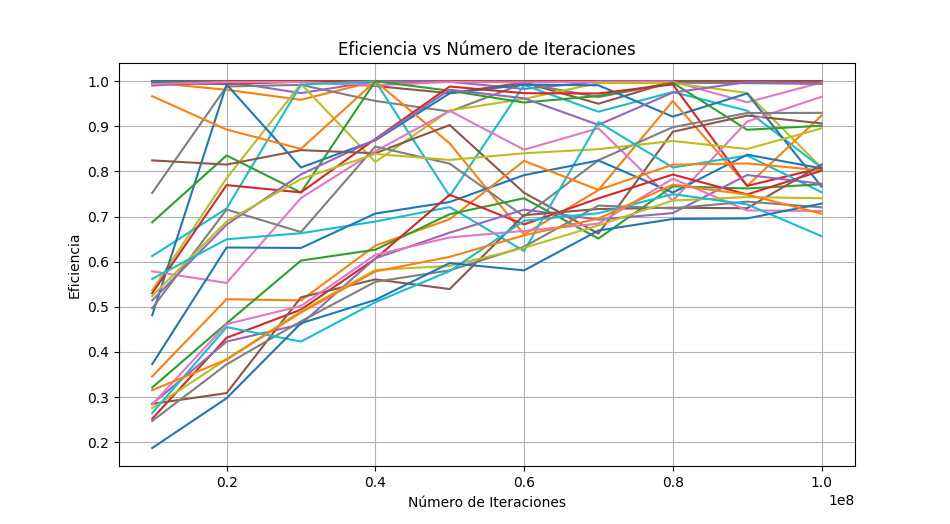
\includegraphics[width=0.45\textwidth]{Figure_4.png}
    \caption{Eficiencia en función del número de iteraciones.}
    \label{fig:eficiencia}
\end{figure}

El gráfico muestra que la eficiencia mejora conforme aumenta el número de iteraciones, aproximándose al valor óptimo de 1 a medida que se incrementa el tamaño del problema. Esto indica que, al distribuir una mayor carga de trabajo entre los procesos, se reduce el impacto del overhead de comunicación, mejorando así la utilización de los recursos paralelos.

Sin embargo, la eficiencia no crece indefinidamente; alcanza un punto en el que se estabiliza e incluso muestra una ligera disminución. Esto se debe a factores como la latencia de comunicación y la sincronización entre procesos, que empiezan a limitar el rendimiento cuando la carga computacional es suficientemente grande para justificar la paralelización, pero no lo suficiente para superar completamente el costo de coordinación.

\begin{figure}[H]
    \centering
    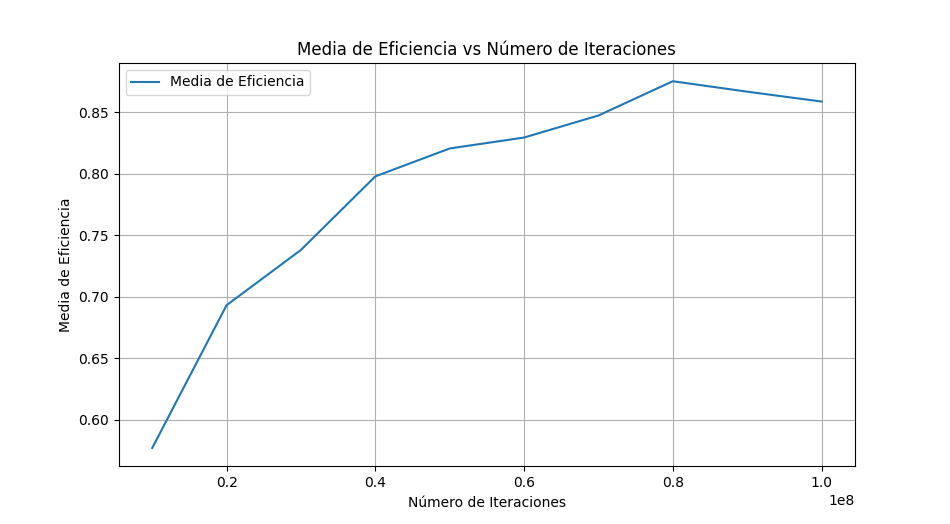
\includegraphics[width=0.45\textwidth]{mediaFigure_4.png}
    \caption{Media Eficiencia en función del número de iteraciones.}
    \label{fig:eficiencia}
\end{figure}

La gráfica de la media de eficiencia confirma esta tendencia. A medida que se incrementa el número de iteraciones, la eficiencia media se aproxima al valor óptimo, alcanzando un equilibrio donde el sistema aprovecha al máximo los recursos paralelos sin incurrir en un overhead significativo. No obstante, el ligero decrecimiento hacia el final sugiere una limitación en la escalabilidad práctica, donde factores como la latencia y la comunicación comienzan a influir.

En resumen, estos resultados sugieren que el método de Monte Carlo distribuido es efectivo y escalable en problemas de gran tamaño, especialmente cuando se dispone de suficientes recursos paralelos. Sin embargo, en configuraciones de ultra-alto rendimiento, la eficiencia puede limitarse por la infraestructura de comunicación, lo cual es importante considerar en aplicaciones que necesiten escalar más allá de los niveles evaluados en esta práctica.

\subsection{Speed-up vs Número de Iteraciones}
\begin{figure}[H]
    \centering
    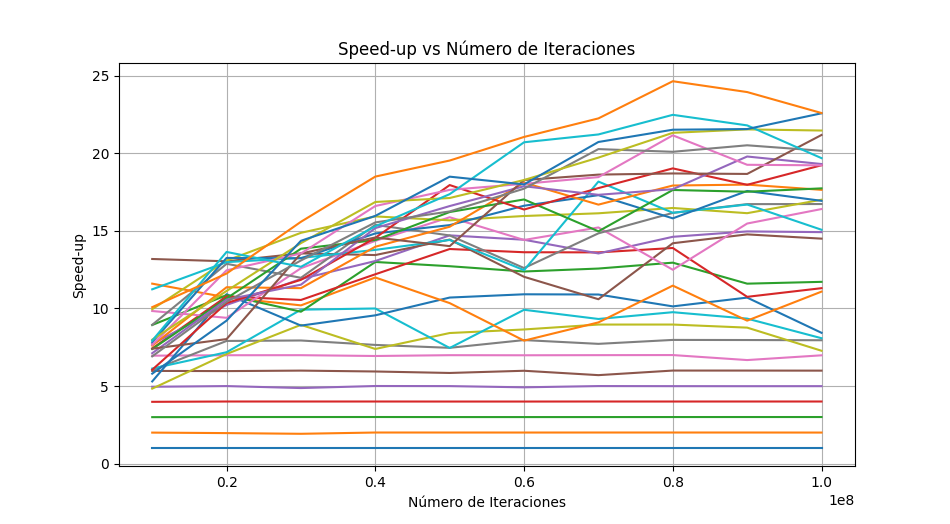
\includegraphics[width=0.45\textwidth]{Figure_3.png}
    \caption{Speed-up en función del número de iteraciones.}
    \label{fig:speedup}
\end{figure}

Se observa que el speed-up aumenta con el número de iteraciones, lo que indica un uso eficiente de los recursos de cálculo. Esta tendencia es particularmente relevante porque demuestra que, al incrementar el tamaño del problema, los procesos paralelos logran reducir el tiempo total de ejecución de manera significativa en comparación con la ejecución secuencial. La gráfica promedio del speed-up (Figura \ref{fig:speedupMedia}) muestra un comportamiento que inicialmente crece de forma constante y sostenida, reflejando un aprovechamiento eficiente de los recursos disponibles.

\begin{figure}[H]
    \centering
    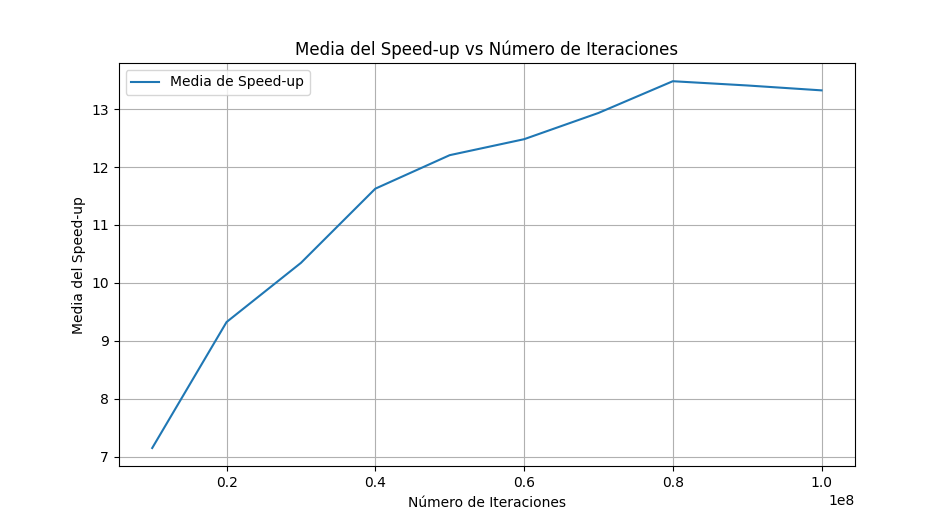
\includegraphics[width=0.45\textwidth]{mediaFigure_3.png}
    \caption{Media Speed-up en función del número de iteraciones.}
    \label{fig:speedupMedia}
\end{figure}

Sin embargo, al analizar la gráfica con la media del speed-up, se aprecia que, después de alcanzar un punto máximo alrededor de \(0.8 \times 10^8\) iteraciones, la mejora empieza a estabilizarse o incluso puede descender levemente. Esto sugiere que, a partir de cierto umbral, la paralelización enfrenta limitaciones debido a la comunicación entre procesos y la sobrecarga de coordinación. Aun así, el hecho de que la media se mantenga alta indica una consistencia en la mejora del rendimiento para tamaños de problema grandes.

Es importante destacar que este comportamiento varía según la configuración del hardware y la cantidad de procesos utilizados. Los sistemas con más núcleos o mejor optimizados pueden extender la región de crecimiento antes de que se alcance la estabilización. 

\subsection{Calidad del Resultado vs Número de Iteraciones}
\begin{figure}[H]
    \centering
    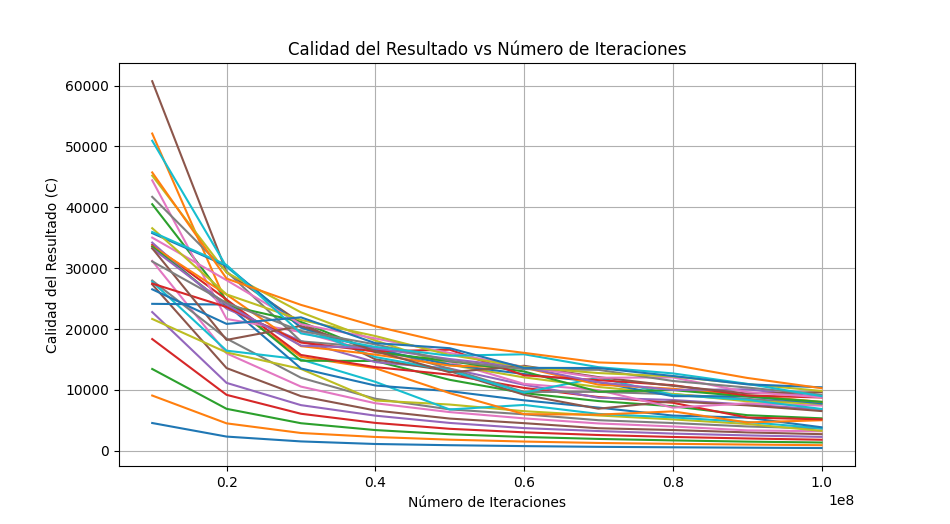
\includegraphics[width=0.45\textwidth]{Figure_2.png}
    \caption{Calidad del resultado en función del número de iteraciones.}
    \label{fig:calidad}
\end{figure}

La gráfica de calidad del resultado muestra que, al aumentar el número de iteraciones, el error en la aproximación de \(\pi\) se estabiliza, reflejando la efectividad del método de Monte Carlo. Al principio, el error es relativamente alto debido a la menor cantidad de puntos de muestreo, lo cual introduce variabilidad en los resultados. Sin embargo, conforme se incrementa el número de iteraciones, esta aleatoriedad se compensa, permitiendo que el método converja de forma más consistente hacia el valor real de \(\pi\) y mantenga una aproximación precisa y estable.

\begin{figure}[H]
    \centering
    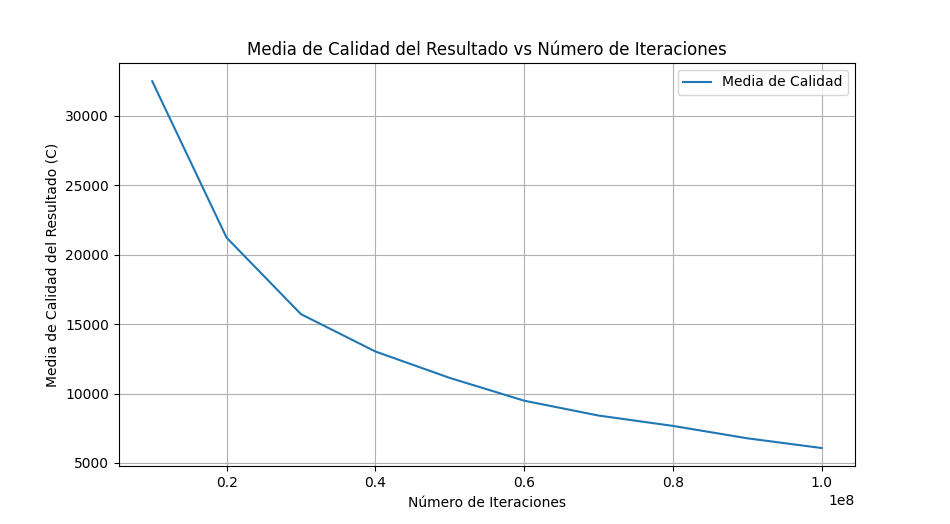
\includegraphics[width=0.45\textwidth]{mediaFigure_2.png}
    \caption{Media Calidad del resultado en función del número de iteraciones.}
    \label{fig:calidad}
\end{figure}

La gráfica de la media de calidad respalda esta tendencia, mostrando una reducción continua del error que se estabiliza en niveles bajos a medida que se alcanzan iteraciones avanzadas. Este comportamiento sugiere que, a partir de un cierto umbral, el aumento en el número de muestras aporta mejoras marginales, indicando que el método ha alcanzado su límite de precisión práctica. En aplicaciones donde el balance entre tiempo de cómputo y precisión es importante, estos resultados ayudan a identificar el número óptimo de iteraciones para maximizar la efectividad del método.


\subsection{Error en la Aproximación de \(\pi\)}
\begin{figure}[H]
    \centering
    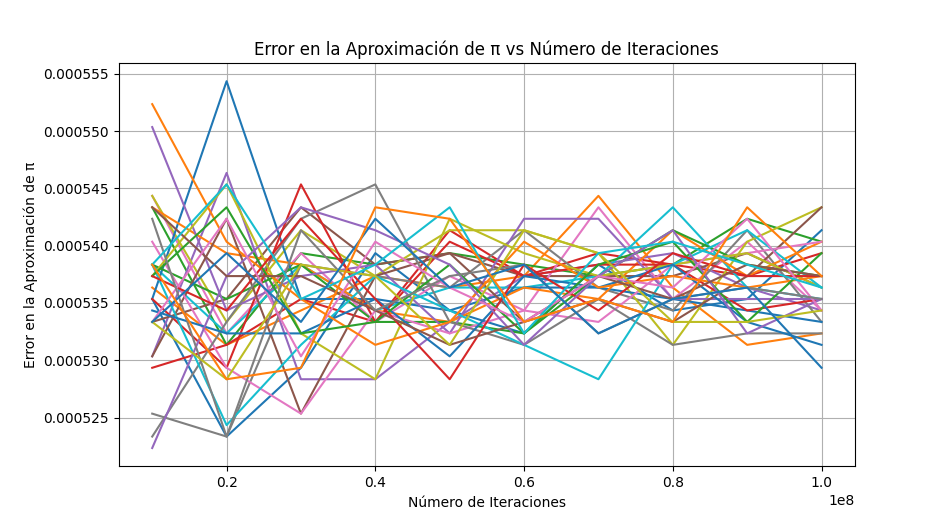
\includegraphics[width=0.45\textwidth]{Figure_1.png}
    \caption{Error en la aproximación de \(\pi\) en función del número de iteraciones.}
    \label{fig:error}
\end{figure}

La gráfica del error en la aproximación de \(\pi\) confirma que el error disminuye y se estabiliza con el incremento de iteraciones, un comportamiento característico de los algoritmos basados en Monte Carlo. A medida que se aumenta el número de puntos de muestreo, las estimaciones convergen hacia el valor real de \(\pi\), reduciendo la dispersión y proporcionando una estimación cada vez más precisa.

\begin{figure}[H]
    \centering
    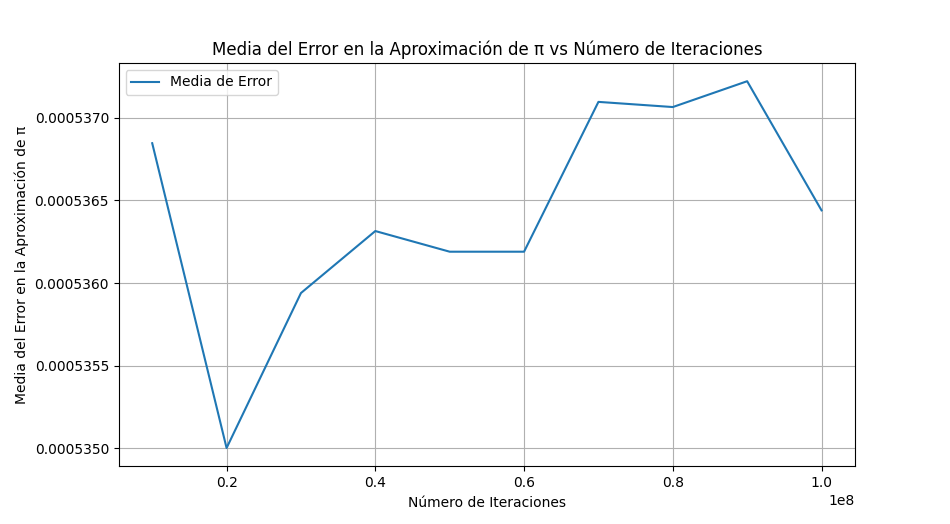
\includegraphics[width=0.45\textwidth]{mediaFigure_1.png}
    \caption{Media Error en la aproximación de \(\pi\) en función del número de iteraciones.}
    \label{fig:error}
\end{figure}

La media del error refleja una tendencia descendente similar, alcanzando un punto de estabilización que marca un umbral de precisión práctica. Esto indica que, aunque el incremento de iteraciones sigue mejorando la precisión, las ganancias se vuelven cada vez más marginales. Este resultado evidencia la robustez del método en términos de convergencia y su efectividad para lograr un equilibrio adecuado entre precisión y tiempo de cálculo en aplicaciones prácticas.

\section{Conclusiones}
El programa implementado para el cálculo de \(\pi\) mediante el método de Monte Carlo, distribuido con MPI, evidencia cómo el incremento del paralelismo contribuye a una mejora significativa en la eficiencia. Al asignar más núcleos para la ejecución de los cálculos, estos pueden realizarse con mayor rapidez. Sin embargo, el uso de un mayor número de núcleos implica una sobrecarga adicional relacionada con la distribución de la carga de trabajo y la sincronización de los resultados, un factor que no se considera en la comparación directa con el programa secuencial. Aun así, debido a la naturaleza computacionalmente intensiva del cálculo iterativo de \(\pi\), el método se beneficia claramente del paralelismo. La estrategia de reducción en árbol binario optimiza la recopilación de datos parciales, minimizando la cantidad de mensajes enviados y reduciendo el overhead de comunicación.

En términos de escalabilidad, los resultados muestran una tendencia clara. A medida que se incrementa la talla del problema, representada en este caso por el número de iteraciones, el uso de un mayor número de núcleos resulta en un aumento significativo del SpeedUp. Esto se debe a que la sobrecarga de comunicación representa una fracción cada vez menor del tiempo total de ejecución, mientras que el tiempo de computación paralela se incrementa proporcionalmente. Sin embargo, esta escalabilidad presenta límites; conforme se añaden más núcleos, el impacto de cada nuevo núcleo en la reducción del tiempo de ejecución disminuye progresivamente, hasta el punto en que el uso adicional de núcleos podría no aportar mejoras sustanciales.

El análisis de las medidas del error sigue un comportamiento esperado desde un punto de vista teórico: el error en la aproximación disminuye a medida que se realizan más iteraciones. No obstante, la relación no es lineal, ya que las iteraciones iniciales tienden a tener un impacto más significativo en la reducción del error. Esto se refleja en las métricas de calidad; aunque el error disminuye con el aumento de las iteraciones, el tiempo de cálculo también crece, y lo hace en una proporción mayor, lo cual reduce la calidad (definida como la inversa del producto entre tiempo y error) conforme se incrementa la carga de trabajo.

En conclusión, el método de Monte Carlo distribuido mediante MPI demuestra ser efectivo y escalable para cálculos intensivos como el de \(\pi\). No obstante, es importante considerar los límites de escalabilidad y la relación no lineal entre la precisión del resultado y el número de iteraciones, aspectos que resultan críticos en la optimización de aplicaciones paralelas en sistemas de gran escala.

\section*{Anexo A: Fórmulas de Aproximación de \(\pi\)}

Las fórmulas de aproximación de \(\pi\) utilizadas en este estudio incluyen una variedad de métodos, desde integrales hasta sumatorias y productorias. A continuación, se listan las fórmulas:

\begin{itemize}
    \item Fórmula de aproximación de \(\pi\) mediante una integral de Gauss:
    \[
    \pi = \left( \int_{-\infty}^{\infty} e^{-x^2} \, dx \right)^2
    \]

    \item Aproximación de \(\pi\) usando una integral de semicírculo:
    \[
    \pi = 4 \int_{0}^{1} \sqrt{1 - x^2} \, dx
    \]

    \item Aproximación de \(\pi\) mediante otra integral de semicírculo:
    \[
    \pi = \int_{-1}^{1} \frac{dx}{\sqrt{1 - x^2}}
    \]

    \item Aproximación de \(\pi\) usando un productorio infinito:
    \[
    \pi = 2 \prod_{k=1}^{\infty} \frac{(2k)^2}{(2k - 1)(2k + 1)}
    \]

    \item Aproximación de \(\pi\) usando una serie infinita:
    \[
    \pi = \sqrt{6 \sum_{k=1}^{\infty} \frac{1}{k^2}}
    \]

    \item Aproximación de \(\pi\) mediante una serie de Machin-like:
    \[
    \pi = \sum_{k=0}^{\infty} \frac{1}{16^k} \left( \frac{4}{8k + 1} - \frac{2}{8k + 4} - \frac{1}{8k + 5} - \frac{1}{8k + 6} \right)
    \]

    \item Aproximación de \(\pi\) mediante una integral:
    \[
    \pi = \frac{22}{7} - \int_{0}^{1} \frac{x^4 (1 - x)^4}{(1 + x)^2} \, dx
    \]

    \item Aproximación de \(\pi\) usando una serie alternada:
    \[
    \pi = 4 \sum_{k=1}^{\infty} \frac{(-1)^{k+1}}{2k - 1}
    \]

    \item Aproximación de \(\pi\) mediante una integral de función racional:
    \[
    \pi = \frac{1}{3} \int_{-3}^{3} \frac{x + 3}{\sqrt{9 - x^2}} \, dx
    \]
\end{itemize}

\section{Análisis de las Gráficas}

\subsection{Media Calidad por Fórmula}

\begin{figure}[h!]
    \centering
    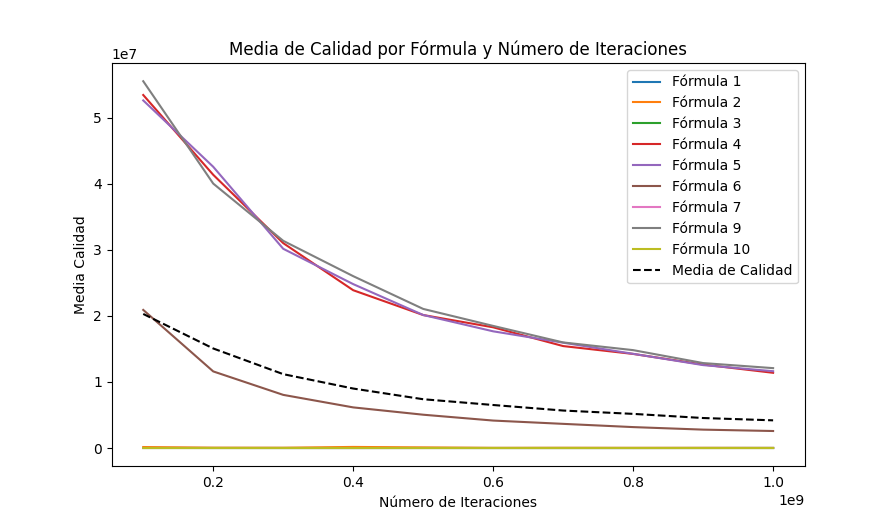
\includegraphics[width=0.45\textwidth]{todasMediaCalidad2.png}
    \caption{Media de la Calidad por fórmula.}
    \label{fig:mediaCalidad}
\end{figure}

La gráfica de la media de calidad en función del número de iteraciones muestra una tendencia decreciente en la calidad conforme se incrementa el número de iteraciones para todas las fórmulas. Esto se debe a que, aunque el error en la aproximación de \(\pi\) disminuye con más iteraciones, el tiempo de cálculo aumenta en mayor proporción, lo cual afecta negativamente la calidad (definida como la inversa del producto entre el tiempo y el error).

Cada fórmula presenta una pendiente decreciente que converge gradualmente hacia un valor bajo de calidad, reflejando que las ganancias en precisión se ven contrarrestadas por el incremento en el tiempo de cómputo. La línea negra discontinua representa la media general de calidad y muestra una tendencia similar, indicando una consistencia en el comportamiento de las fórmulas independientemente de las particularidades de cada una.

Al analizar la gráfica, observamos que la fórmula 10 presenta la mejor calidad, ya que mantiene valores de calidad consistentemente más altos en comparación con las demás, lo cual sugiere que logra un buen equilibrio entre precisión y tiempo de cálculo. Por otro lado, la fórmula 3 muestra la peor calidad, con valores significativamente más bajos que el resto de las fórmulas, indicando que requiere más tiempo para alcanzar un nivel de precisión comparable, afectando así su rendimiento en términos de calidad.

\subsection{Media de Eficiencia por Fórmula}

\begin{figure}[h!]
    \centering
    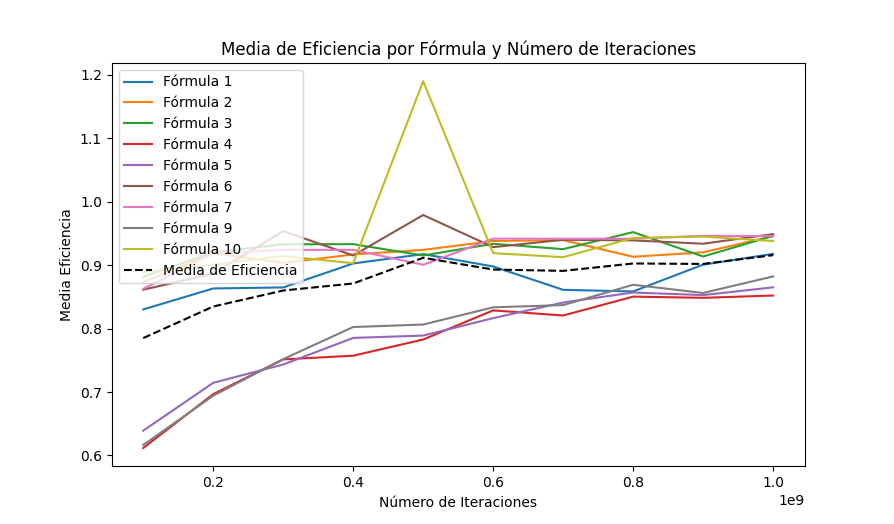
\includegraphics[width=0.45\textwidth]{todasMediaEficiencia2.png}
    \caption{Media de la Eficiencia por fórmula.}
    \label{fig:mediaEficiencia}
\end{figure}

La gráfica de eficiencia muestra cómo las fórmulas alcanzan niveles de eficiencia cercanos al óptimo (valor de 1) en altos números de iteraciones. Al principio, algunas fórmulas presentan variaciones en la eficiencia debido al overhead inicial asociado a la comunicación y sincronización entre procesos. A medida que el número de iteraciones aumenta, la mayoría de las fórmulas convergen hacia una eficiencia estable, alrededor del óptimo.

Algunas fórmulas muestran picos de eficiencia que superan el valor de 1 debido a posibles efectos en la configuración de hardware y optimizaciones específicas del cálculo en entornos paralelos. La media de eficiencia, representada por la línea discontinua, confirma que el sistema se mantiene eficiente en configuraciones de gran tamaño, pero tiende a estabilizarse, lo que implica un límite práctico en la escalabilidad del método.

En esta gráfica, se observa que la fórmula 2 logra la mejor eficiencia, manteniendo valores cercanos o incluso superiores al óptimo de manera más consistente que otras fórmulas, lo que sugiere una menor carga de overhead y un aprovechamiento eficiente de los recursos en configuraciones paralelas. Por otro lado, la fórmula 7 presenta la peor eficiencia, mostrando valores más bajos a lo largo de todas las iteraciones y convergiendo a un nivel de eficiencia inferior al resto, lo cual indica que su implementación podría estar más afectada por el overhead y los costos de sincronización.

\subsection{Media de Error por Fórmula}

\begin{figure}[h!]
    \centering
    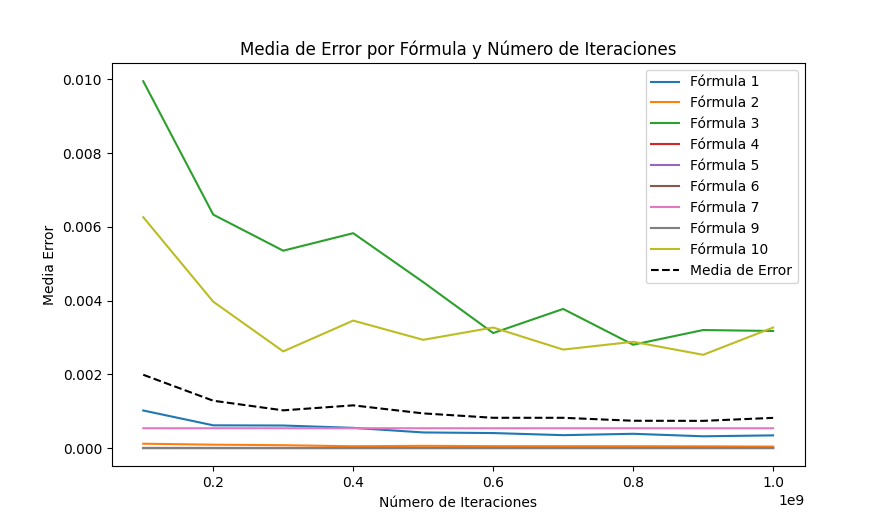
\includegraphics[width=0.45\textwidth]{todasMediaError2.png}
    \caption{Media del Error por fórmula.}
    \label{fig:mediaError}
\end{figure}

La gráfica de error muestra una disminución progresiva en el error conforme aumenta el número de iteraciones, lo cual es coherente con las expectativas teóricas de los métodos iterativos. Las fórmulas de aproximación convergen a diferentes tasas, reflejando la precisión inherente de cada método.

En particular, algunas fórmulas, como la fórmula 3 y la fórmula 9, presentan un error inicial más alto, que disminuye gradualmente con el aumento en las iteraciones. En contraste, otras fórmulas muestran un error significativamente bajo desde el inicio y se mantienen estables. La línea discontinua que representa la media del error confirma una tendencia decreciente general en todas las fórmulas, estabilizándose en niveles bajos de error en iteraciones avanzadas, lo cual indica que se ha alcanzado un umbral de precisión práctica.

Al analizar los resultados, observamos que la fórmula 5 logra la mejor precisión, manteniendo consistentemente los niveles de error más bajos en todas las iteraciones, lo que la hace muy efectiva en términos de exactitud desde las primeras iteraciones. Por otro lado, la fórmula 3 es la que presenta el peor rendimiento en cuanto a error, ya que empieza con valores significativamente más altos y muestra una disminución más lenta, lo que sugiere que requiere muchas más iteraciones para alcanzar un nivel de precisión comparable.

\subsection{Media de Speedup por Fórmula}

\begin{figure}[h!]
    \centering
    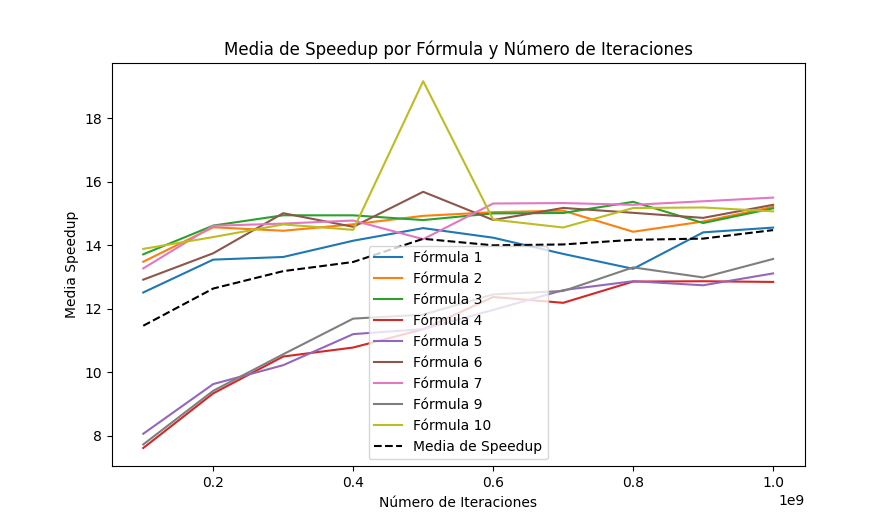
\includegraphics[width=0.45\textwidth]{todasMediaSpeedup.png}
    \caption{Media del Speedup por fórmula.}
    \label{fig:mediaError}
\end{figure}

La gráfica de speedup muestra un incremento a medida que se aumenta el número de iteraciones, lo que indica que el paralelismo resulta en una reducción significativa del tiempo de cálculo en comparación con la ejecución secuencial. Sin embargo, similar a la eficiencia, algunas fórmulas experimentan picos de speedup en ciertos puntos, lo que podría deberse a optimizaciones específicas en el cálculo o a variaciones en la distribución de carga.

La línea discontinua que representa la media de speedup sugiere un aumento gradual en el rendimiento, alcanzando un nivel estable en altos números de iteraciones. Esto refleja una buena escalabilidad para la mayoría de las fórmulas, aunque con limitaciones, ya que el speedup no sigue creciendo indefinidamente.

Al observar la gráfica, se destaca que la fórmula 2 alcanza el mejor speedup, manteniendo consistentemente valores más altos en comparación con las otras fórmulas. Esto indica que es particularmente efectiva en aprovechar el paralelismo y reducir el tiempo de cálculo conforme aumenta la carga de trabajo. Por el contrario, la fórmula 7 muestra el peor rendimiento en términos de speedup, con valores más bajos y menos consistentes a lo largo de las iteraciones, lo cual sugiere que su escalabilidad está limitada y que no aprovecha de manera óptima los recursos paralelos.

\subsection{Conslusiones}

El análisis comparativo de las diferentes fórmulas para la aproximación de \(\pi\) en un entorno paralelo ha revelado variaciones significativas en términos de calidad, eficiencia, error y speedup. Cada fórmula muestra fortalezas y debilidades específicas, lo cual es crucial para determinar su adecuación a distintos escenarios de cálculo paralelo intensivo.

La fórmula 10 ha demostrado ser la mejor en términos de calidad, logrando un equilibrio óptimo entre precisión y tiempo de cálculo en comparación con las demás fórmulas. Este rendimiento superior en calidad sugiere que la fórmula 10 es particularmente útil en situaciones donde se requiere un alto grado de precisión sin sacrificar rendimiento computacional. Por otro lado, la fórmula 3 mostró la peor calidad, con un tiempo de cálculo significativamente mayor en relación con la precisión alcanzada, lo que la hace menos eficiente para aplicaciones que demanden resultados rápidos y precisos.

En cuanto a la eficiencia, la fórmula 2 ha destacado al alcanzar y mantener valores cercanos o incluso superiores al óptimo en múltiples configuraciones de iteraciones. Esto implica que la fórmula 2 es menos afectada por el overhead de sincronización y aprovecha eficientemente el paralelismo, haciéndola ideal para entornos donde la maximización del uso de los recursos paralelos es esencial. En contraste, la fórmula 7 tuvo un desempeño significativamente inferior en términos de eficiencia, lo cual indica una mayor sensibilidad al overhead y a los costos de comunicación, limitando su escalabilidad y rendimiento en configuraciones paralelas grandes.

Respecto al error, la fórmula 5 se consolidó como la más precisa, logrando bajos niveles de error desde las primeras iteraciones. Esta consistencia en precisión hace que la fórmula 5 sea ideal para aplicaciones donde la exactitud es una prioridad. La fórmula 3, nuevamente, presentó el peor rendimiento en términos de error, mostrando una convergencia más lenta y necesitando muchas más iteraciones para alcanzar un nivel de precisión comparable al de otras fórmulas.

Finalmente, en términos de speedup, la fórmula 2 mostró el mejor rendimiento, manteniendo altos valores de speedup de manera consistente a lo largo de las iteraciones. Esto indica que es particularmente efectiva en reducir el tiempo de cálculo conforme aumenta la carga de trabajo, maximizando así los beneficios del paralelismo. La fórmula 7, en cambio, obtuvo el peor speedup, con un desempeño más irregular y valores más bajos, lo que sugiere que no aprovecha de manera óptima los recursos paralelos disponibles.

En conclusión, este análisis comparativo revela que la elección de la fórmula adecuada depende de los objetivos específicos de la aplicación. Para maximizar la calidad y la eficiencia, las fórmulas 10 y 2 son las opciones más recomendables, respectivamente. Si el objetivo es minimizar el error, la fórmula 5 ofrece los mejores resultados. Por otro lado, la fórmula 3 resulta menos adecuada para aplicaciones que requieran eficiencia y precisión rápidas, mientras que la fórmula 7 muestra limitaciones significativas en términos de escalabilidad y aprovechamiento del paralelismo. Este análisis proporciona una guía para seleccionar la fórmula de aproximación de \(\pi\) más adecuada según los requisitos de precisión, eficiencia y escalabilidad en aplicaciones de computación paralela intensiva.

\end{document}